%!TEX root=icsme2016-mccurdyc.tex
% mainfile: icsme2016-mccurdyc.tex

\documentclass[hyperref]{beamer}

\usecolortheme[accent=blue,dark]{solarized}

\beamertemplatetransparentcovered

\usepackage[utf8]{inputenc}
\usepackage{merriweather}
\usepackage{moresize}
\usepackage{anyfontsize}
\usepackage{xcolor}
\usepackage{graphicx}
\usepackage{subcaption}
\usepackage{fontawesome}
\usepackage{booktabs}
\usepackage{adjustbox}
\usepackage{array}
\usepackage{subcaption}

\usepackage{pgfplots}
\pgfplotsset{compat=1.9}
\usepgfplotslibrary{colormaps,external}

\usepackage{pifont}
\newcommand{\cmark}{{\color{solarizedGreen}\ding{51}}}
\newcommand{\xmark}{{\color{solarizedRed}{\ding{55}}}}
\newcommand{\cmarkhide}{{\color{solarizedBase2}\ding{51}}}
\newcommand{\xmarkhide}{{\color{solarizedBase2}{\ding{55}}}}
% \newcommand{\cmark}{{\color{solarizedGreen}\ding{51}}}
% \newcommand{\xmark}{{\color{solarizedOrange}{\ding{55}}}}
% \newcommand{\cmarkhide}{{\color{kapfhammerDarkGrey}\ding{51}}}
% \newcommand{\xmarkhide}{{\color{kapfhammerDarkGrey}{\ding{55}}}}
\newcommand\sql[1]{{\tt \small #1}}


%% Rotated table column type
\newcolumntype{R}[2]{%
    >{\adjustbox{minipage=6em,angle=#1,lap=\width-(#2)}\bgroup}%
    l%
    <{\egroup}%
}
\newcommand*\rot{\multicolumn{1}{R{40}{3em}}}

\usepackage{tikz}
\usetikzlibrary{positioning,shadows,arrows,shapes,calc,backgrounds}

\setbeamercolor{background canvas}{bg=solarizedBase2}
% \setbeamercolor{background canvas}{bg=kapfhammerDarkGrey}

\setbeamertemplate{section in toc shaded}[default][65]
\setbeamertemplate{subsection in toc shaded}[default][65]

\setbeamertemplate{navigation symbols}{}

\setbeamerfont{title}{size=\HUGE,series=\rmfamily,parent=merriweather}
% \setbeamerfont{title}{size=\Huge,series=\rmfamily,parent=merriweather}
\setbeamerfont{frametitle}{size=\HUGE,series=\rmfamily,parent=merriweather}
\setbeamerfont{framesubtitle}{size=\normalsize,series=\rmfamily,parent=merriweather}
\setbeamerfont{subtitle}{size=\normalsize,series=\bfseries,parent=merriweather}
\setbeamerfont{author}{size=\LARGE,series=\bfseries,parent=merriweather}
\setbeamerfont{institute}{size=\normalsize,series=\bfseries,parent=merriweather}
\setbeamerfont{date}{size=\normalsize,series=\bfseries,parent=merriweather}

\setbeamercolor{title}{fg=solarizedBlue}
% \setbeamercolor{title}{fg=solarizedOrange}
\setbeamercolor{subtitle}{fg=solarizedOrange}
% \setbeamercolor{subtitle}{fg=solarizedViolet}
\setbeamercolor{frametitle}{fg=solarizedBase02}
\setbeamercolor{framesubtitle}{fg=solarizedBase02}
% \setbeamercolor{frametitle}{fg=kapfhammerDarkGrey}
% \setbeamercolor{framesubtitle}{fg=kapfhammerDarkGrey}
\setbeamercolor{author}{fg=solarizedRebase00}
\setbeamercolor{institute}{fg=solarizedRebase00}
\setbeamercolor{date}{fg=solarizedRebase00}

\addtobeamertemplate{frametitle}{\vskip.1in}{}

\graphicspath{ {images/} }

\usepackage{listings}

\title{\fontsize{50}{50}\selectfont{mrstudyr}}
\subtitle{Retrospective Mutant Reduction}

\author[McCurdy]{Colton J. McCurdy\\
{\small \href{https://twitter.com/McCurdyColton}{\textcolor{solarizedOrange}{\fontsize{15}{30}{\faTwitter\,}\small McCurdyColton}}}}
\institute[ICSME 2016]{ICSME 2016}
\date[September 23, 2016]{October 6, 2016}

\begin{document}

\begin{frame}
  \titlepage
\end{frame}

\section{Motivation}
%!TEX root=icsme2016-mccurdyc.tex
% mainfile: icsme2016-mccurdyc.tex

  \begin{frame}
    \frametitle{Motivation}
    \begin{center}
    \HUGE{Why are we here?}
    \end{center}
  \end{frame}


\setbeamercovered{invisible}
\begin{frame}%[label=current]
  \frametitle{Motivation}

  % \vspace*{.3in}
  % \begin{center}
  %   \fontsize{90}{72}\selectfont
  %   O(\uncover<2->{\textcolor{solarizedViolet}{?}})
  % \end{center}

 \tikzstyle{proc} = [draw, thick, fill=solarizedViolet, text centered, rounded corners,
    text=solarizedRebase02, draw=solarizedViolet]

\tikzstyle{prochighlight} = [draw, thick, fill=solarizedOrange, text centered, rounded corners,
    text=solarizedRebase02, draw=solarizedOrange]

\tikzstyle{procold} = [draw, thick, fill=solarizedViolet!75, text centered, rounded corners,
    text=solarizedRebase02, draw=solarizedViolet!75]

\tikzstyle{procchanged} = [draw, thick, fill=solarizedViolet!75, text centered, rounded corners,
    text=solarizedRebase02, draw=solarizedViolet!75]

\tikzstyle{prochighlightold} = [draw, thick, fill=solarizedOrange!75, text centered, rounded corners,
    text=solarizedRebase02, draw=solarizedOrange!75]

\tikzstyle{prochighlightchanged} = [draw, thick, fill=solarizedYellow!75, text centered, rounded corners,
    text=solarizedRebase02, draw=solarizedYellow!75]

\tikzstyle{proctest} = [draw, thick, fill=solarizedOrange, text centered, rounded corners,
text=solarizedBase02, draw=solarizedOrange]

\tikzstyle{procnew} = [draw, thick, fill=solarizedGreen, text centered, rounded corners,
    text=solarizedRebase02, draw=solarizedGreen]

\tikzstyle{procyellow} = [draw, thick, fill=solarizedYellow, text centered, rounded corners,
    text=solarizedRebase02, draw=solarizedYellow]

\tikzstyle{procred} = [draw, thick, fill=solarizedRed, text centered, rounded corners,
    text=solarizedRebase02, draw=solarizedRed]

\tikzstyle{io} = [ellipse, draw, thick, fill=solarizedBlue, draw=solarizedBlue, text=solarizedRebase02]

\tikzstyle{iopass} = [ellipse, draw, thick, fill=solarizedGreen, draw=solarizedGreen, text=solarizedRebase02]
\tikzstyle{iofail} = [ellipse, draw, thick, fill=solarizedRed, draw=solarizedRed, text=solarizedRebase02]
\tikzstyle{iohighlight} = [ellipse, draw, thick, fill=solarizedYellow, draw=solarizedYellow,
    text=solarizedRebase02]

\tikzstyle{iofailother} = [ellipse, draw, thick, fill=solarizedYellow, draw=solarizedYellow,
    text=solarizedRebase02]
\tikzstyle{wrongoutput} = [ellipse, draw, thick, fill=solarizedCyan, draw=solarizedCyan, text=solarizedRebase02]

\tikzstyle{special} = [draw, thick, fill=solarizedGreen, text centered, draw=solarizedGreen,
    text=solarizedBase02]
\tikzstyle{specialOrange} = [draw, thick, fill=solarizedOrange, text centered, draw=solarizedOrange,
    text=solarizedBase02]
\tikzstyle{specialGreen} = [draw, thick, fill=solarizedGreen, text centered, draw=solarizedGreen,
    text=solarizedBase02]
\tikzstyle{specialYellow} = [draw, thick, fill=solarizedYellow, text centered, draw=solarizedYellow,
    text=solarizedBase02]

\tikzstyle{pass} = [draw, thick, fill=solarizedGreen, text centered, draw=solarizedGreen, text=solarizedRebase02]
\tikzstyle{fail} = [draw, thick, fill=solarizedRed, text centered, draw=solarizedRed, text=solarizedRebase02]

\tikzstyle{feature} = [draw, thick, fill=solarizedOrange, text centered, text=solarizedRebase02, draw=solarizedOrange]

\tikzstyle{plain} = [draw, thick, fill=solarizedBase2, text centered, text=solarizedRebase1, draw=solarizedBase2]
\tikzstyle{featurecurve} = [draw, thick, fill=solarizedGreen, text centered, rounded corners]

 \begin{figure}[!htb]
    \centering
    \begin{minipage}{0.5\textwidth}
        \centering
          \begin{tikzpicture}[node distance=0cm, auto,>=stealth, thick]

        \path[fill=black!25, rounded corners, draw=black] (0,0) rectangle (4,-5);
        \draw[solarizedViolet, line width=5pt] (0.25,-0.5) -- (2,-0.5);
        \draw[solarizedOrange, line width=5pt] (0.25,-1) -- (3,-1);
        \draw[solarizedBlue, line width=5pt] (0.25,-1.5) -- (2.5,-1.5);

        \draw[solarizedViolet, line width=5pt] (0.25,-2.5) -- (2,-2.5);
        \draw[solarizedOrange, line width=5pt] (0.25,-3) -- (3.75,-3);
        \draw[solarizedBlue, line width=5pt] (0.25,-3.5) -- (3.5,-3.5);

        \draw[solarizedViolet, line width=5pt] (0.25,-4.5) -- (3,-4.5);


\end{tikzpicture}

        \begin{tikzpicture}
          \path[->]<1> node[plain, text width=20ex]
          (Pass) at (-2.75,-.25) {\Huge \cmarkhide {Pass}};

          \path[->]<2-> node[plain, text width=20ex]
          (Pass) at (-2.75,-.25) {\Huge \cmark {Pass}};
        \end{tikzpicture}
    \end{minipage}%
    \begin{minipage}{0.5\textwidth}
        \centering
        \begin{tikzpicture}[node distance=0cm, auto,>=stealth, thick]

        \path[fill=black!15, rounded corners, draw=black] (0,0) rectangle (4,-5);
        \draw[solarizedOrange, line width=5pt] (0.25,-0.5) -- (2,-0.5);
        \draw[solarizedBlue, line width=5pt] (0.25,-1) -- (1,-1);
        \draw[solarizedViolet, line width=5pt] (0.25,-1.5) -- (3.5,-1.5);
        \draw[solarizedBlue, line width=5pt] (0.25,-2) -- (2,-2);
        \draw[solarizedRed, line width=5pt] (0.25,-2.5) -- (3.75,-2.5);

        \draw[solarizedOrange, line width=5pt] (0.25,-3.5) -- (3.75,-3.5);
        \draw[solarizedBlue, line width=5pt] (0.25,-4) -- (1.75,-4);
        \draw[solarizedViolet, line width=5pt] (0.25,-4.5) -- (2.5,-4.5);



\end{tikzpicture}

       \begin{tikzpicture}
          \path[->]<1> node[plain, text width=20ex,
          yshift=-0.0in, xshift=1.75in, minimum width=20ex]
          (Fail) {\Huge \xmarkhide {Fail}};

          \path[->]<2> node[plain, text width=20ex,
          yshift=-0.0in, xshift=1.75in, minimum width=20ex]
          (Fail) {\Huge \xmarkhide {Fail}};

          \path[->]<3-> node[plain, text width=20ex,
          yshift=-0.0in, xshift=1.75in, minimum width=20ex]
          (Fail) {\Huge \xmark {Fail}};
        \end{tikzpicture}
    \end{minipage}
\end{figure}
\end{frame}

  \begin{frame}
    \frametitle{Motivation}
    \begin{center}
    \HUGE{Merit?}
    \end{center}
  \end{frame}


\section{Background}
  \begin{frame}
    \frametitle{Background}
    \begin{center}
        {\fontsize{50}{50}\selectfont{Mutation Testing!}}
    \end{center}
  \end{frame}

  \begin{frame}
      % TODO: I want to add a "tagline" at the bottom just saying the significance of square corners
    \frametitle{Mutation Testing}
 \tikzstyle{proc} = [draw, thick, fill=solarizedViolet, text centered, rounded corners,
    text=solarizedRebase02, draw=solarizedViolet]

\tikzstyle{prochighlight} = [draw, thick, fill=solarizedOrange, text centered, rounded corners,
    text=solarizedRebase02, draw=solarizedOrange]

\tikzstyle{procold} = [draw, thick, fill=solarizedViolet!75, text centered, rounded corners,
    text=solarizedRebase02, draw=solarizedViolet!75]

\tikzstyle{procchanged} = [draw, thick, fill=solarizedViolet!75, text centered, rounded corners,
    text=solarizedRebase02, draw=solarizedViolet!75]

\tikzstyle{prochighlightold} = [draw, thick, fill=solarizedOrange!75, text centered, rounded corners,
    text=solarizedRebase02, draw=solarizedOrange!75]

\tikzstyle{prochighlightchanged} = [draw, thick, fill=solarizedYellow!75, text centered, rounded corners,
    text=solarizedRebase02, draw=solarizedYellow!75]

\tikzstyle{proctest} = [draw, thick, fill=solarizedOrange, text centered, rounded corners,
text=solarizedBase02, draw=solarizedOrange]

\tikzstyle{procnew} = [draw, thick, fill=solarizedGreen, text centered, rounded corners,
    text=solarizedRebase02, draw=solarizedGreen]

\tikzstyle{procyellow} = [draw, thick, fill=solarizedYellow, text centered, rounded corners,
    text=solarizedRebase02, draw=solarizedYellow]

\tikzstyle{procred} = [draw, thick, fill=solarizedRed, text centered, rounded corners,
    text=solarizedRebase02, draw=solarizedRed]

\tikzstyle{io} = [ellipse, draw, thick, fill=solarizedBlue, draw=solarizedBlue, text=solarizedRebase02]

\tikzstyle{iopass} = [ellipse, draw, thick, fill=solarizedGreen, draw=solarizedGreen, text=solarizedRebase02]
\tikzstyle{iofail} = [ellipse, draw, thick, fill=solarizedRed, draw=solarizedRed, text=solarizedRebase02]
\tikzstyle{iohighlight} = [ellipse, draw, thick, fill=solarizedYellow, draw=solarizedYellow,
    text=solarizedRebase02]

\tikzstyle{iofailother} = [ellipse, draw, thick, fill=solarizedYellow, draw=solarizedYellow,
    text=solarizedRebase02]
\tikzstyle{wrongoutput} = [ellipse, draw, thick, fill=solarizedCyan, draw=solarizedCyan, text=solarizedRebase02]

\tikzstyle{special} = [draw, thick, fill=solarizedGreen, text centered, draw=solarizedGreen,
    text=solarizedBase02]
\tikzstyle{specialOrange} = [draw, thick, fill=solarizedOrange, text centered, draw=solarizedOrange,
    text=solarizedBase02]
\tikzstyle{specialGreen} = [draw, thick, fill=solarizedGreen, text centered, draw=solarizedGreen,
    text=solarizedBase02]
\tikzstyle{specialYellow} = [draw, thick, fill=solarizedYellow, text centered, draw=solarizedYellow,
    text=solarizedBase02]

\tikzstyle{pass} = [draw, thick, fill=solarizedGreen, text centered, draw=solarizedGreen, text=solarizedRebase02]
\tikzstyle{fail} = [draw, thick, fill=solarizedRed, text centered, draw=solarizedRed, text=solarizedRebase02]

\tikzstyle{feature} = [draw, thick, fill=solarizedOrange, text centered, text=solarizedRebase02, draw=solarizedOrange]

\tikzstyle{plain} = [draw, thick, fill=solarizedBase2, text centered, text=solarizedRebase1, draw=solarizedBase2]
\tikzstyle{featurecurve} = [draw, thick, fill=solarizedGreen, text centered, rounded corners]

 \begin{figure}[!htb]
    \centering
    \begin{minipage}{0.5\textwidth}
        \centering
          \begin{tikzpicture}[node distance=0cm, auto,>=stealth, thick]

        \path[fill=black!15, draw=solarizedBase02] (0,0) rectangle (4,-5);
        \draw[solarizedViolet, line width=5pt] (0.25,-0.5) -- (2,-0.5);
        \draw[solarizedOrange, line width=5pt] (0.25,-1) -- (3,-1);
        \draw[solarizedBlue, line width=5pt] (0.25,-1.5) -- (2.5,-1.5);

        \draw[solarizedViolet, line width=5pt] (0.25,-2.5) -- (2,-2.5);
        \draw[solarizedOrange, line width=5pt] (0.25,-3) -- (3.75,-3);
        \draw[solarizedBlue, line width=5pt] (0.25,-3.5) -- (3.5,-3.5);

        \draw[solarizedViolet, line width=5pt] (0.25,-4.5) -- (3,-4.5);


\end{tikzpicture}

        \begin{tikzpicture}
          \path[->]<1> node[plain, text width=20ex]
          (Pass) at (-2.75,-.25) {\Huge Original};
        \end{tikzpicture}
    \end{minipage}%
    \begin{minipage}{0.5\textwidth}
        \centering
        \vspace*{-0.8em} % issue with text under box
        \begin{tikzpicture}[node distance=0cm, auto,>=stealth, thick]

        \path[fill=black!15, draw=solarizedBase02] (0,0) rectangle (4,-5);
        \draw[solarizedViolet, line width=5pt] (0.25,-0.5) -- (2,-0.5);
        \draw[solarizedOrange, line width=5pt] (0.25,-1) -- (3,-1);
        \draw[solarizedBlue, line width=5pt] (0.25,-1.5) -- (2.5,-1.5);

        \draw[solarizedViolet, line width=5pt] (0.25,-2.5) -- (2,-2.5);
        \draw[solarizedOrange, line width=5pt] (0.25,-3) -- (3.75,-3);
        \draw[solarizedBlue, line width=5pt] (0.25,-3.5) -- (3.5,-3.5);
        \draw[yellow, line width=5pt] (1.25,-3.5) -- (2.75,-3.5);

        \draw[solarizedViolet, line width=5pt] (0.25,-4.5) -- (3,-4.5);


\end{tikzpicture}

       \begin{tikzpicture}
          \path[->]<1> node[plain, text width=20ex,
          yshift=0.0in, xshift=1.75in, minimum width=20ex]
          (Mutant) {\Huge Mutant};
        \end{tikzpicture}
    \end{minipage}
\end{figure}
\end{frame}

  \begin{frame}
    \frametitle{Mutation Testing}
 \tikzstyle{proc} = [draw, thick, fill=solarizedViolet, text centered, rounded corners,
    text=solarizedRebase02, draw=solarizedViolet]

\tikzstyle{prochighlight} = [draw, thick, fill=solarizedOrange, text centered, rounded corners,
    text=solarizedRebase02, draw=solarizedOrange]

\tikzstyle{procold} = [draw, thick, fill=solarizedViolet!75, text centered, rounded corners,
    text=solarizedRebase02, draw=solarizedViolet!75]

\tikzstyle{procchanged} = [draw, thick, fill=solarizedViolet!75, text centered, rounded corners,
    text=solarizedRebase02, draw=solarizedViolet!75]

\tikzstyle{prochighlightold} = [draw, thick, fill=solarizedOrange!75, text centered, rounded corners,
    text=solarizedRebase02, draw=solarizedOrange!75]

\tikzstyle{prochighlightchanged} = [draw, thick, fill=solarizedYellow!75, text centered, rounded corners,
    text=solarizedRebase02, draw=solarizedYellow!75]

\tikzstyle{proctest} = [draw, thick, fill=solarizedOrange, text centered, rounded corners,
text=solarizedBase02, draw=solarizedOrange]

\tikzstyle{procnew} = [draw, thick, fill=solarizedGreen, text centered, rounded corners,
    text=solarizedRebase02, draw=solarizedGreen]

\tikzstyle{procyellow} = [draw, thick, fill=solarizedYellow, text centered, rounded corners,
    text=solarizedRebase02, draw=solarizedYellow]

\tikzstyle{procred} = [draw, thick, fill=solarizedRed, text centered, rounded corners,
    text=solarizedRebase02, draw=solarizedRed]

\tikzstyle{io} = [ellipse, draw, thick, fill=solarizedBlue, draw=solarizedBlue, text=solarizedRebase02]

\tikzstyle{iopass} = [ellipse, draw, thick, fill=solarizedGreen, draw=solarizedGreen, text=solarizedRebase02]
\tikzstyle{iofail} = [ellipse, draw, thick, fill=solarizedRed, draw=solarizedRed, text=solarizedRebase02]
\tikzstyle{iohighlight} = [ellipse, draw, thick, fill=solarizedYellow, draw=solarizedYellow,
    text=solarizedRebase02]

\tikzstyle{iofailother} = [ellipse, draw, thick, fill=solarizedYellow, draw=solarizedYellow,
    text=solarizedRebase02]
\tikzstyle{wrongoutput} = [ellipse, draw, thick, fill=solarizedCyan, draw=solarizedCyan, text=solarizedRebase02]

\tikzstyle{special} = [draw, thick, fill=solarizedGreen, text centered, draw=solarizedGreen,
    text=solarizedBase02]
\tikzstyle{specialOrange} = [draw, thick, fill=solarizedOrange, text centered, draw=solarizedOrange,
    text=solarizedBase02]
\tikzstyle{specialGreen} = [draw, thick, fill=solarizedGreen, text centered, draw=solarizedGreen,
    text=solarizedBase02]
\tikzstyle{specialYellow} = [draw, thick, fill=solarizedYellow, text centered, draw=solarizedYellow,
    text=solarizedBase02]

\tikzstyle{pass} = [draw, thick, fill=solarizedGreen, text centered, draw=solarizedGreen, text=solarizedRebase02]
\tikzstyle{fail} = [draw, thick, fill=solarizedRed, text centered, draw=solarizedRed, text=solarizedRebase02]

\tikzstyle{feature} = [draw, thick, fill=solarizedOrange, text centered, text=solarizedRebase02, draw=solarizedOrange]

\tikzstyle{plain} = [draw, thick, fill=solarizedBase2, text centered, text=solarizedRebase1, draw=solarizedBase2]
\tikzstyle{featurecurve} = [draw, thick, fill=solarizedGreen, text centered, rounded corners]

 \begin{figure}[!htb]
    \centering
    \begin{minipage}{0.5\textwidth}
        \centering
          \begin{tikzpicture}[node distance=0cm, auto,>=stealth, thick]

        \path[fill=black!15, draw=solarizedBase02] (0,0) rectangle (4,-5);
        \draw[solarizedViolet, line width=5pt] (0.25,-0.5) -- (2,-0.5);
        \draw[solarizedOrange, line width=5pt] (0.25,-1) -- (3,-1);
        \draw[solarizedBlue, line width=5pt] (0.25,-1.5) -- (2.5,-1.5);

        \draw[solarizedViolet, line width=5pt] (0.25,-2.5) -- (2,-2.5);
        \draw[solarizedOrange, line width=5pt] (0.25,-3) -- (3.75,-3);
        \draw[solarizedBlue, line width=5pt] (0.25,-3.5) -- (3.5,-3.5);

        \draw[solarizedViolet, line width=5pt] (0.25,-4.5) -- (3,-4.5);


\end{tikzpicture}

        \begin{tikzpicture}
          \path[->]<1> node[plain, text width=20ex]
          (Pass) at (-2.75,-.25) {\Huge Original};
        \end{tikzpicture}
    \end{minipage}%
    \begin{minipage}{0.5\textwidth}
        \centering
        \vspace*{-0.8em} % issue with text under box
        \begin{tikzpicture}[node distance=0cm, auto,>=stealth, thick]

        \path[fill=black!15, draw=solarizedBase02] (0,0) rectangle (4,-5);
        \draw[solarizedViolet, line width=5pt] (0.25,-0.5) -- (2,-0.5);
        \draw[solarizedOrange, line width=5pt] (0.25,-1) -- (3,-1);
        \draw[solarizedBlue, line width=5pt] (0.25,-1.5) -- (2.5,-1.5);

        \draw[solarizedViolet, line width=5pt] (0.25,-2.5) -- (2,-2.5);
        \draw[solarizedOrange, line width=5pt] (0.25,-3) -- (3.75,-3);
        \draw[solarizedBlue, line width=5pt] (0.25,-3.5) -- (3.5,-3.5);
        \draw[yellow, line width=5pt] (1.25,-3.5) -- (2.75,-3.5);
        \path[rounded corners, draw=solarizedRed, line width=5pt] (1,-3) rectangle (3,-4);

        \draw[solarizedViolet, line width=5pt] (0.25,-4.5) -- (3,-4.5);


\end{tikzpicture}

       \begin{tikzpicture}
          \path[->]<1> node[plain, text width=20ex,
          yshift=0.0in, xshift=1.75in, minimum width=20ex]
          (Mutant) {\Huge Mutant};
        \end{tikzpicture}
    \end{minipage}
\end{figure}
\end{frame}

  \begin{frame}
    \frametitle{Mutation Testing}
    % \begin{center}
        % {\HUGE Mutant?} \\
        \begin{tikzpicture}[node distance=0cm, auto,>=stealth, thick]


    \tikzstyle{box}=[rectangle, draw=solarizedBase02, rounded corners, fill=solarizedBlue, drop shadow,
            text centered, anchor=north, text=white, minimum height = 1cm, text width=3cm]
    \tikzstyle{operator}=[rectangle, draw=solarizedBase02, rounded corners, fill=solarizedOrange, drop shadow,
            text centered, anchor=north, text=white, minimum height = 1cm, text width=8cm]
    \tikzstyle{smallbox}=[rectangle, draw=solarizedBase02, rounded corners, fill=solarizedBlue, drop shadow,
            text centered, anchor=north, text=white, minimum height = 1cm, text width=2cm]

            \visible<1->{\node (op) [box] {a \textcolor{yellow}{$<$ op $>$} \textcolor{white}{b}};}
            \visible<2->{\node (operator) [operator, below = 1cm of op] {Conditional Operator Replacement (COR)};}
            \visible<3->{\node (op1) [smallbox] at (-4.25cm, -4cm) {a \&\& b};}
            \visible<3->{\node (op2) [smallbox, right = 0.5cm of op1] {a $||$ b};}
            \visible<4->{\node (op3) [smallbox, right = 0.5cm of op2] {a == b};}
            \visible<4->{\node (op4) [smallbox, right = 0.5cm of op3] {a != b};}

            % TODO: Fix overlapping arrows
            \visible<2->{\draw[->, line width = 3pt] (op) -- (operator);}
            \visible<3->{\draw[->, line width = 3pt] (operator) -- (op1);}
            \visible<3->{\draw[->, line width = 3pt] (operator) -- (op2);}
            \visible<4->{\draw[->, line width = 3pt] (operator) -- (op3);}
            \visible<4->{\draw[->, line width = 3pt] (operator) -- (op4);}

\end{tikzpicture}

    % \end{center}
  \end{frame}

  \begin{frame}
    \frametitle{Mutation Testing}
 \tikzstyle{proc} = [draw, thick, fill=solarizedViolet, text centered, rounded corners,
    text=solarizedRebase02, draw=solarizedViolet]

\tikzstyle{prochighlight} = [draw, thick, fill=solarizedOrange, text centered, rounded corners,
    text=solarizedRebase02, draw=solarizedOrange]

\tikzstyle{procold} = [draw, thick, fill=solarizedViolet!75, text centered, rounded corners,
    text=solarizedRebase02, draw=solarizedViolet!75]

\tikzstyle{procchanged} = [draw, thick, fill=solarizedViolet!75, text centered, rounded corners,
    text=solarizedRebase02, draw=solarizedViolet!75]

\tikzstyle{prochighlightold} = [draw, thick, fill=solarizedOrange!75, text centered, rounded corners,
    text=solarizedRebase02, draw=solarizedOrange!75]

\tikzstyle{prochighlightchanged} = [draw, thick, fill=solarizedYellow!75, text centered, rounded corners,
    text=solarizedRebase02, draw=solarizedYellow!75]

\tikzstyle{proctest} = [draw, thick, fill=solarizedOrange, text centered, rounded corners,
text=solarizedBase02, draw=solarizedOrange]

\tikzstyle{procnew} = [draw, thick, fill=solarizedGreen, text centered, rounded corners,
    text=solarizedRebase02, draw=solarizedGreen]

\tikzstyle{procyellow} = [draw, thick, fill=solarizedYellow, text centered, rounded corners,
    text=solarizedRebase02, draw=solarizedYellow]

\tikzstyle{procred} = [draw, thick, fill=solarizedRed, text centered, rounded corners,
    text=solarizedRebase02, draw=solarizedRed]

\tikzstyle{io} = [ellipse, draw, thick, fill=solarizedBlue, draw=solarizedBlue, text=solarizedRebase02]

\tikzstyle{iopass} = [ellipse, draw, thick, fill=solarizedGreen, draw=solarizedGreen, text=solarizedRebase02]
\tikzstyle{iofail} = [ellipse, draw, thick, fill=solarizedRed, draw=solarizedRed, text=solarizedRebase02]
\tikzstyle{iohighlight} = [ellipse, draw, thick, fill=solarizedYellow, draw=solarizedYellow,
    text=solarizedRebase02]

\tikzstyle{iofailother} = [ellipse, draw, thick, fill=solarizedYellow, draw=solarizedYellow,
    text=solarizedRebase02]
\tikzstyle{wrongoutput} = [ellipse, draw, thick, fill=solarizedCyan, draw=solarizedCyan, text=solarizedRebase02]

\tikzstyle{special} = [draw, thick, fill=solarizedGreen, text centered, draw=solarizedGreen,
    text=solarizedBase02]
\tikzstyle{specialOrange} = [draw, thick, fill=solarizedOrange, text centered, draw=solarizedOrange,
    text=solarizedBase02]
\tikzstyle{specialGreen} = [draw, thick, fill=solarizedGreen, text centered, draw=solarizedGreen,
    text=solarizedBase02]
\tikzstyle{specialYellow} = [draw, thick, fill=solarizedYellow, text centered, draw=solarizedYellow,
    text=solarizedBase02]

\tikzstyle{pass} = [draw, thick, fill=solarizedGreen, text centered, draw=solarizedGreen, text=solarizedRebase02]
\tikzstyle{fail} = [draw, thick, fill=solarizedRed, text centered, draw=solarizedRed, text=solarizedRebase02]

\tikzstyle{feature} = [draw, thick, fill=solarizedOrange, text centered, text=solarizedRebase02, draw=solarizedOrange]

\tikzstyle{plain} = [draw, thick, fill=solarizedBase2, text centered, text=solarizedRebase1, draw=solarizedBase2]
\tikzstyle{featurecurve} = [draw, thick, fill=solarizedGreen, text centered, rounded corners]

 \begin{figure}[!htb]
    \centering
    \begin{minipage}{0.5\textwidth}
        \centering
          \begin{tikzpicture}[node distance=0cm, auto,>=stealth, thick]

        \path[fill=black!15, draw=solarizedBase02] (0,0) rectangle (4,-5);
        \draw[solarizedViolet, line width=5pt] (0.25,-0.5) -- (2,-0.5);
        \draw[solarizedOrange, line width=5pt] (0.25,-1) -- (3,-1);
        \draw[solarizedBlue, line width=5pt] (0.25,-1.5) -- (2.5,-1.5);

        \draw[solarizedViolet, line width=5pt] (0.25,-2.5) -- (2,-2.5);
        \draw[solarizedOrange, line width=5pt] (0.25,-3) -- (3.75,-3);
        \draw[solarizedBlue, line width=5pt] (0.25,-3.5) -- (3.5,-3.5);
        \draw[yellow, line width=5pt] (1.25,-3.5) -- (2.75,-3.5);

        \draw[solarizedViolet, line width=5pt] (0.25,-4.5) -- (3,-4.5);


\end{tikzpicture}

        \begin{tikzpicture}
          \path[->]<1> node[plain, text width=20ex]
          (Alive) at (-2.75,-.25) {\Huge \cmarkhide {Alive}};

          \path[->]<2-> node[plain, text width=20ex]
          (Alive) at (-2.75,-.25) {\Huge \cmark {Alive}};
        \end{tikzpicture}
    \end{minipage}%
    \begin{minipage}{0.5\textwidth}
        \centering
        \begin{tikzpicture}[node distance=0cm, auto,>=stealth, thick]

        \path[fill=black!15, draw=solarizedBase02] (0,0) rectangle (4,-5);
        \draw[solarizedViolet, line width=5pt] (0.25,-0.5) -- (2,-0.5);
        \draw[solarizedOrange, line width=5pt] (0.25,-1) -- (3,-1);
        \draw[solarizedBlue, line width=5pt] (0.25,-1.5) -- (2.5,-1.5);

        \draw[solarizedViolet, line width=5pt] (0.25,-2.5) -- (2,-2.5);
        \draw[solarizedOrange, line width=5pt] (0.25,-3) -- (3.75,-3);
        \draw[solarizedBlue, line width=5pt] (0.25,-3.5) -- (3.5,-3.5);
        \draw[yellow, line width=5pt] (1.25,-3.5) -- (2.75,-3.5);

        \draw[solarizedViolet, line width=5pt] (0.25,-4.5) -- (3,-4.5);


\end{tikzpicture}

       \begin{tikzpicture}
          \path[->]<1> node[plain, text width=20ex,
          yshift=0.0in, xshift=1.75in, minimum width=20ex]
          (Killed) {\Huge \xmarkhide {Killed}};

          \path[->]<2> node[plain, text width=20ex,
          yshift=-0.0in, xshift=1.75in, minimum width=20ex]
          (Killed) {\Huge \xmarkhide {Killed}};
        \end{tikzpicture}
    \end{minipage}
\end{figure}
\end{frame}

  \begin{frame}
    \frametitle{Mutation Testing}
 \tikzstyle{proc} = [draw, thick, fill=solarizedViolet, text centered, rounded corners,
    text=solarizedRebase02, draw=solarizedViolet]

\tikzstyle{prochighlight} = [draw, thick, fill=solarizedOrange, text centered, rounded corners,
    text=solarizedRebase02, draw=solarizedOrange]

\tikzstyle{procold} = [draw, thick, fill=solarizedViolet!75, text centered, rounded corners,
    text=solarizedRebase02, draw=solarizedViolet!75]

\tikzstyle{procchanged} = [draw, thick, fill=solarizedViolet!75, text centered, rounded corners,
    text=solarizedRebase02, draw=solarizedViolet!75]

\tikzstyle{prochighlightold} = [draw, thick, fill=solarizedOrange!75, text centered, rounded corners,
    text=solarizedRebase02, draw=solarizedOrange!75]

\tikzstyle{prochighlightchanged} = [draw, thick, fill=solarizedYellow!75, text centered, rounded corners,
    text=solarizedRebase02, draw=solarizedYellow!75]

\tikzstyle{proctest} = [draw, thick, fill=solarizedOrange, text centered, rounded corners,
text=solarizedBase02, draw=solarizedOrange]

\tikzstyle{procnew} = [draw, thick, fill=solarizedGreen, text centered, rounded corners,
    text=solarizedRebase02, draw=solarizedGreen]

\tikzstyle{procyellow} = [draw, thick, fill=solarizedYellow, text centered, rounded corners,
    text=solarizedRebase02, draw=solarizedYellow]

\tikzstyle{procred} = [draw, thick, fill=solarizedRed, text centered, rounded corners,
    text=solarizedRebase02, draw=solarizedRed]

\tikzstyle{io} = [ellipse, draw, thick, fill=solarizedBlue, draw=solarizedBlue, text=solarizedRebase02]

\tikzstyle{iopass} = [ellipse, draw, thick, fill=solarizedGreen, draw=solarizedGreen, text=solarizedRebase02]
\tikzstyle{iofail} = [ellipse, draw, thick, fill=solarizedRed, draw=solarizedRed, text=solarizedRebase02]
\tikzstyle{iohighlight} = [ellipse, draw, thick, fill=solarizedYellow, draw=solarizedYellow,
    text=solarizedRebase02]

\tikzstyle{iofailother} = [ellipse, draw, thick, fill=solarizedYellow, draw=solarizedYellow,
    text=solarizedRebase02]
\tikzstyle{wrongoutput} = [ellipse, draw, thick, fill=solarizedCyan, draw=solarizedCyan, text=solarizedRebase02]

\tikzstyle{special} = [draw, thick, fill=solarizedGreen, text centered, draw=solarizedGreen,
    text=solarizedBase02]
\tikzstyle{specialOrange} = [draw, thick, fill=solarizedOrange, text centered, draw=solarizedOrange,
    text=solarizedBase02]
\tikzstyle{specialGreen} = [draw, thick, fill=solarizedGreen, text centered, draw=solarizedGreen,
    text=solarizedBase02]
\tikzstyle{specialYellow} = [draw, thick, fill=solarizedYellow, text centered, draw=solarizedYellow,
    text=solarizedBase02]

\tikzstyle{pass} = [draw, thick, fill=solarizedGreen, text centered, draw=solarizedGreen, text=solarizedRebase02]
\tikzstyle{fail} = [draw, thick, fill=solarizedRed, text centered, draw=solarizedRed, text=solarizedRebase02]

\tikzstyle{feature} = [draw, thick, fill=solarizedOrange, text centered, text=solarizedRebase02, draw=solarizedOrange]

\tikzstyle{plain} = [draw, thick, fill=solarizedBase2, text centered, text=solarizedRebase1, draw=solarizedBase2]
\tikzstyle{featurecurve} = [draw, thick, fill=solarizedGreen, text centered, rounded corners]

 \begin{figure}[!htb]
    \centering
    \begin{minipage}{0.5\textwidth}
        \centering
          \begin{tikzpicture}[node distance=0cm, auto,>=stealth, thick]

        \path[fill=black!15, draw=solarizedBase02] (0,0) rectangle (4,-5);
        \draw[solarizedViolet, line width=5pt] (0.25,-0.5) -- (2,-0.5);
        \draw[solarizedOrange, line width=5pt] (0.25,-1) -- (3,-1);
        \draw[solarizedBlue, line width=5pt] (0.25,-1.5) -- (2.5,-1.5);

        \draw[solarizedViolet, line width=5pt] (0.25,-2.5) -- (2,-2.5);
        \draw[solarizedOrange, line width=5pt] (0.25,-3) -- (3.75,-3);
        \draw[solarizedBlue, line width=5pt] (0.25,-3.5) -- (3.5,-3.5);
        \draw[yellow, line width=5pt] (1.25,-3.5) -- (2.75,-3.5);

        \draw[solarizedViolet, line width=5pt] (0.25,-4.5) -- (3,-4.5);


\end{tikzpicture}

        \begin{tikzpicture}
          \path[->] node[plain, text width=20ex]
          (Alive) at (-2.75,-.25) {\Huge \cmark {Alive}};

        \end{tikzpicture}
    \end{minipage}%
    \begin{minipage}{0.5\textwidth}
        \centering
        \begin{tikzpicture}[node distance=0cm, auto,>=stealth, thick]

        \path[fill=black!15, draw=solarizedBase02] (0,0) rectangle (4,-5);
        \draw[solarizedViolet, line width=5pt] (0.25,-0.5) -- (2,-0.5);
        \draw[solarizedOrange, line width=5pt] (0.25,-1) -- (3,-1);
        \draw[solarizedBlue, line width=5pt] (0.25,-1.5) -- (2.5,-1.5);

        \draw[solarizedViolet, line width=5pt] (0.25,-2.5) -- (2,-2.5);
        \draw[solarizedOrange, line width=5pt] (0.25,-3) -- (3.75,-3);
        \draw[solarizedBlue, line width=5pt] (0.25,-3.5) -- (3.5,-3.5);
        \draw[yellow, line width=5pt] (1.25,-3.5) -- (2.75,-3.5);
        \path[rounded corners, draw=solarizedRed, line width=5pt] (1,-3) rectangle (3,-4);
        \draw[solarizedRed, line width=5pt] (1,-3) -- (3,-4);
        \draw[solarizedRed, line width=5pt] (1,-4) -- (3,-3);

        \draw[solarizedViolet, line width=5pt] (0.25,-4.5) -- (3,-4.5);


\end{tikzpicture}

       \begin{tikzpicture}
          \path[->]<1-> node[plain, text width=20ex,
          yshift=-0.0in, xshift=1.75in, minimum width=20ex]
          (Killed) {\Huge \xmarkhide {Killed}};

          \path[->]<2-> node[plain, text width=20ex,
          yshift=-0.0in, xshift=1.75in, minimum width=20ex]
          (Killed) {\Huge \xmark {Killed}};
        \end{tikzpicture}
    \end{minipage}
\end{figure}
\end{frame}

  \begin{frame}
    \frametitle{Mutation Testing}
    \tikzstyle{proc} = [draw, thick, fill=solarizedViolet, text centered, rounded corners,
    text=solarizedRebase02, draw=solarizedViolet]

\tikzstyle{prochighlight} = [draw, thick, fill=solarizedOrange, text centered, rounded corners,
    text=solarizedRebase02, draw=solarizedOrange]

\tikzstyle{procold} = [draw, thick, fill=solarizedViolet!75, text centered, rounded corners,
    text=solarizedRebase02, draw=solarizedViolet!75]

\tikzstyle{procchanged} = [draw, thick, fill=solarizedViolet!75, text centered, rounded corners,
    text=solarizedRebase02, draw=solarizedViolet!75]

\tikzstyle{prochighlightold} = [draw, thick, fill=solarizedOrange!75, text centered, rounded corners,
    text=solarizedRebase02, draw=solarizedOrange!75]

\tikzstyle{prochighlightchanged} = [draw, thick, fill=solarizedYellow!75, text centered, rounded corners,
    text=solarizedRebase02, draw=solarizedYellow!75]

\tikzstyle{proctest} = [draw, thick, fill=solarizedOrange, text centered, rounded corners,
text=solarizedBase02, draw=solarizedOrange]

\tikzstyle{procnew} = [draw, thick, fill=solarizedGreen, text centered, rounded corners,
    text=solarizedRebase02, draw=solarizedGreen]

\tikzstyle{procyellow} = [draw, thick, fill=solarizedYellow, text centered, rounded corners,
    text=solarizedRebase02, draw=solarizedYellow]

\tikzstyle{procred} = [draw, thick, fill=solarizedRed, text centered, rounded corners,
    text=solarizedRebase02, draw=solarizedRed]

\tikzstyle{io} = [ellipse, draw, thick, fill=solarizedBlue, draw=solarizedBlue, text=solarizedRebase02]

\tikzstyle{iopass} = [ellipse, draw, thick, fill=solarizedGreen, draw=solarizedGreen, text=solarizedRebase02]
\tikzstyle{iofail} = [ellipse, draw, thick, fill=solarizedRed, draw=solarizedRed, text=solarizedRebase02]
\tikzstyle{iohighlight} = [ellipse, draw, thick, fill=solarizedYellow, draw=solarizedYellow,
    text=solarizedRebase02]

\tikzstyle{iofailother} = [ellipse, draw, thick, fill=solarizedYellow, draw=solarizedYellow,
    text=solarizedRebase02]
\tikzstyle{wrongoutput} = [ellipse, draw, thick, fill=solarizedCyan, draw=solarizedCyan, text=solarizedRebase02]

\tikzstyle{special} = [draw, thick, fill=solarizedGreen, text centered, draw=solarizedGreen,
    text=solarizedBase02]
\tikzstyle{specialOrange} = [draw, thick, fill=solarizedOrange, text centered, draw=solarizedOrange,
    text=solarizedBase02]
\tikzstyle{specialGreen} = [draw, thick, fill=solarizedGreen, text centered, draw=solarizedGreen,
    text=solarizedBase02]
\tikzstyle{specialYellow} = [draw, thick, fill=solarizedYellow, text centered, draw=solarizedYellow,
    text=solarizedBase02]

\tikzstyle{pass} = [draw, thick, fill=solarizedGreen, text centered, draw=solarizedGreen, text=solarizedRebase02]
\tikzstyle{fail} = [draw, thick, fill=solarizedRed, text centered, draw=solarizedRed, text=solarizedRebase02]

\tikzstyle{feature} = [draw, thick, fill=solarizedOrange, text centered, text=solarizedRebase02, draw=solarizedOrange]

\tikzstyle{plain} = [draw, thick, fill=solarizedBase2, text centered, text=solarizedRebase1, draw=solarizedBase2]
\tikzstyle{featurecurve} = [draw, thick, fill=solarizedGreen, text centered, rounded corners]

    \begin{figure}[!htb]
    \centering
        \centering
        \vspace*{-3.5cm}
        {\fontsize{50}{50}\selectfont{$$MS_T = \frac{Killed}{Total}$$}}
    \end{figure}
    \end{frame}

  \begin{frame}
    \frametitle{Mutation Testing}
    \tikzstyle{proc} = [draw, thick, fill=solarizedViolet, text centered, rounded corners,
    text=solarizedRebase02, draw=solarizedViolet]

\tikzstyle{prochighlight} = [draw, thick, fill=solarizedOrange, text centered, rounded corners,
    text=solarizedRebase02, draw=solarizedOrange]

\tikzstyle{procold} = [draw, thick, fill=solarizedViolet!75, text centered, rounded corners,
    text=solarizedRebase02, draw=solarizedViolet!75]

\tikzstyle{procchanged} = [draw, thick, fill=solarizedViolet!75, text centered, rounded corners,
    text=solarizedRebase02, draw=solarizedViolet!75]

\tikzstyle{prochighlightold} = [draw, thick, fill=solarizedOrange!75, text centered, rounded corners,
    text=solarizedRebase02, draw=solarizedOrange!75]

\tikzstyle{prochighlightchanged} = [draw, thick, fill=solarizedYellow!75, text centered, rounded corners,
    text=solarizedRebase02, draw=solarizedYellow!75]

\tikzstyle{proctest} = [draw, thick, fill=solarizedOrange, text centered, rounded corners,
text=solarizedBase02, draw=solarizedOrange]

\tikzstyle{procnew} = [draw, thick, fill=solarizedGreen, text centered, rounded corners,
    text=solarizedRebase02, draw=solarizedGreen]

\tikzstyle{procyellow} = [draw, thick, fill=solarizedYellow, text centered, rounded corners,
    text=solarizedRebase02, draw=solarizedYellow]

\tikzstyle{procred} = [draw, thick, fill=solarizedRed, text centered, rounded corners,
    text=solarizedRebase02, draw=solarizedRed]

\tikzstyle{io} = [ellipse, draw, thick, fill=solarizedBlue, draw=solarizedBlue, text=solarizedRebase02]

\tikzstyle{iopass} = [ellipse, draw, thick, fill=solarizedGreen, draw=solarizedGreen, text=solarizedRebase02]
\tikzstyle{iofail} = [ellipse, draw, thick, fill=solarizedRed, draw=solarizedRed, text=solarizedRebase02]
\tikzstyle{iohighlight} = [ellipse, draw, thick, fill=solarizedYellow, draw=solarizedYellow,
    text=solarizedRebase02]

\tikzstyle{iofailother} = [ellipse, draw, thick, fill=solarizedYellow, draw=solarizedYellow,
    text=solarizedRebase02]
\tikzstyle{wrongoutput} = [ellipse, draw, thick, fill=solarizedCyan, draw=solarizedCyan, text=solarizedRebase02]

\tikzstyle{special} = [draw, thick, fill=solarizedGreen, text centered, draw=solarizedGreen,
    text=solarizedBase02]
\tikzstyle{specialOrange} = [draw, thick, fill=solarizedOrange, text centered, draw=solarizedOrange,
    text=solarizedBase02]
\tikzstyle{specialGreen} = [draw, thick, fill=solarizedGreen, text centered, draw=solarizedGreen,
    text=solarizedBase02]
\tikzstyle{specialYellow} = [draw, thick, fill=solarizedYellow, text centered, draw=solarizedYellow,
    text=solarizedBase02]

\tikzstyle{pass} = [draw, thick, fill=solarizedGreen, text centered, draw=solarizedGreen, text=solarizedRebase02]
\tikzstyle{fail} = [draw, thick, fill=solarizedRed, text centered, draw=solarizedRed, text=solarizedRebase02]

\tikzstyle{feature} = [draw, thick, fill=solarizedOrange, text centered, text=solarizedRebase02, draw=solarizedOrange]

\tikzstyle{plain} = [draw, thick, fill=solarizedBase2, text centered, text=solarizedRebase1, draw=solarizedBase2]
\tikzstyle{featurecurve} = [draw, thick, fill=solarizedGreen, text centered, rounded corners]

    \begin{figure}[!htb]
    \centering
        \centering
        \vspace*{-3.5cm}
        {\fontsize{50}{50}\selectfont{$$MS_T = \frac{Killed}{\textcolor{solarizedViolet}{Total}}$$}}
    \end{figure}
    \end{frame}

  \begin{frame}
    \frametitle{Mutation Testing}
    \tikzstyle{proc} = [draw, thick, fill=solarizedViolet, text centered, rounded corners,
    text=solarizedRebase02, draw=solarizedViolet]

\tikzstyle{prochighlight} = [draw, thick, fill=solarizedOrange, text centered, rounded corners,
    text=solarizedRebase02, draw=solarizedOrange]

\tikzstyle{procold} = [draw, thick, fill=solarizedViolet!75, text centered, rounded corners,
    text=solarizedRebase02, draw=solarizedViolet!75]

\tikzstyle{procchanged} = [draw, thick, fill=solarizedViolet!75, text centered, rounded corners,
    text=solarizedRebase02, draw=solarizedViolet!75]

\tikzstyle{prochighlightold} = [draw, thick, fill=solarizedOrange!75, text centered, rounded corners,
    text=solarizedRebase02, draw=solarizedOrange!75]

\tikzstyle{prochighlightchanged} = [draw, thick, fill=solarizedYellow!75, text centered, rounded corners,
    text=solarizedRebase02, draw=solarizedYellow!75]

\tikzstyle{proctest} = [draw, thick, fill=solarizedOrange, text centered, rounded corners,
text=solarizedBase02, draw=solarizedOrange]

\tikzstyle{procnew} = [draw, thick, fill=solarizedGreen, text centered, rounded corners,
    text=solarizedRebase02, draw=solarizedGreen]

\tikzstyle{procyellow} = [draw, thick, fill=solarizedYellow, text centered, rounded corners,
    text=solarizedRebase02, draw=solarizedYellow]

\tikzstyle{procred} = [draw, thick, fill=solarizedRed, text centered, rounded corners,
    text=solarizedRebase02, draw=solarizedRed]

\tikzstyle{io} = [ellipse, draw, thick, fill=solarizedBlue, draw=solarizedBlue, text=solarizedRebase02]

\tikzstyle{iopass} = [ellipse, draw, thick, fill=solarizedGreen, draw=solarizedGreen, text=solarizedRebase02]
\tikzstyle{iofail} = [ellipse, draw, thick, fill=solarizedRed, draw=solarizedRed, text=solarizedRebase02]
\tikzstyle{iohighlight} = [ellipse, draw, thick, fill=solarizedYellow, draw=solarizedYellow,
    text=solarizedRebase02]

\tikzstyle{iofailother} = [ellipse, draw, thick, fill=solarizedYellow, draw=solarizedYellow,
    text=solarizedRebase02]
\tikzstyle{wrongoutput} = [ellipse, draw, thick, fill=solarizedCyan, draw=solarizedCyan, text=solarizedRebase02]

\tikzstyle{special} = [draw, thick, fill=solarizedGreen, text centered, draw=solarizedGreen,
    text=solarizedBase02]
\tikzstyle{specialOrange} = [draw, thick, fill=solarizedOrange, text centered, draw=solarizedOrange,
    text=solarizedBase02]
\tikzstyle{specialGreen} = [draw, thick, fill=solarizedGreen, text centered, draw=solarizedGreen,
    text=solarizedBase02]
\tikzstyle{specialYellow} = [draw, thick, fill=solarizedYellow, text centered, draw=solarizedYellow,
    text=solarizedBase02]

\tikzstyle{pass} = [draw, thick, fill=solarizedGreen, text centered, draw=solarizedGreen, text=solarizedRebase02]
\tikzstyle{fail} = [draw, thick, fill=solarizedRed, text centered, draw=solarizedRed, text=solarizedRebase02]

\tikzstyle{feature} = [draw, thick, fill=solarizedOrange, text centered, text=solarizedRebase02, draw=solarizedOrange]

\tikzstyle{plain} = [draw, thick, fill=solarizedBase2, text centered, text=solarizedRebase1, draw=solarizedBase2]
\tikzstyle{featurecurve} = [draw, thick, fill=solarizedGreen, text centered, rounded corners]

    \begin{figure}[!htb]
    \centering
        \centering
        \vspace*{-3.5cm}
        {\fontsize{50}{50}\selectfont{$$MS_T = \frac{\textcolor{solarizedViolet}{Killed}}{Total}$$}}
    \end{figure}
    \end{frame}

  \begin{frame}
    \frametitle{Mutation Testing}
    \tikzstyle{proc} = [draw, thick, fill=solarizedViolet, text centered, rounded corners,
    text=solarizedRebase02, draw=solarizedViolet]

\tikzstyle{prochighlight} = [draw, thick, fill=solarizedOrange, text centered, rounded corners,
    text=solarizedRebase02, draw=solarizedOrange]

\tikzstyle{procold} = [draw, thick, fill=solarizedViolet!75, text centered, rounded corners,
    text=solarizedRebase02, draw=solarizedViolet!75]

\tikzstyle{procchanged} = [draw, thick, fill=solarizedViolet!75, text centered, rounded corners,
    text=solarizedRebase02, draw=solarizedViolet!75]

\tikzstyle{prochighlightold} = [draw, thick, fill=solarizedOrange!75, text centered, rounded corners,
    text=solarizedRebase02, draw=solarizedOrange!75]

\tikzstyle{prochighlightchanged} = [draw, thick, fill=solarizedYellow!75, text centered, rounded corners,
    text=solarizedRebase02, draw=solarizedYellow!75]

\tikzstyle{proctest} = [draw, thick, fill=solarizedOrange, text centered, rounded corners,
text=solarizedBase02, draw=solarizedOrange]

\tikzstyle{procnew} = [draw, thick, fill=solarizedGreen, text centered, rounded corners,
    text=solarizedRebase02, draw=solarizedGreen]

\tikzstyle{procyellow} = [draw, thick, fill=solarizedYellow, text centered, rounded corners,
    text=solarizedRebase02, draw=solarizedYellow]

\tikzstyle{procred} = [draw, thick, fill=solarizedRed, text centered, rounded corners,
    text=solarizedRebase02, draw=solarizedRed]

\tikzstyle{io} = [ellipse, draw, thick, fill=solarizedBlue, draw=solarizedBlue, text=solarizedRebase02]

\tikzstyle{iopass} = [ellipse, draw, thick, fill=solarizedGreen, draw=solarizedGreen, text=solarizedRebase02]
\tikzstyle{iofail} = [ellipse, draw, thick, fill=solarizedRed, draw=solarizedRed, text=solarizedRebase02]
\tikzstyle{iohighlight} = [ellipse, draw, thick, fill=solarizedYellow, draw=solarizedYellow,
    text=solarizedRebase02]

\tikzstyle{iofailother} = [ellipse, draw, thick, fill=solarizedYellow, draw=solarizedYellow,
    text=solarizedRebase02]
\tikzstyle{wrongoutput} = [ellipse, draw, thick, fill=solarizedCyan, draw=solarizedCyan, text=solarizedRebase02]

\tikzstyle{special} = [draw, thick, fill=solarizedGreen, text centered, draw=solarizedGreen,
    text=solarizedBase02]
\tikzstyle{specialOrange} = [draw, thick, fill=solarizedOrange, text centered, draw=solarizedOrange,
    text=solarizedBase02]
\tikzstyle{specialGreen} = [draw, thick, fill=solarizedGreen, text centered, draw=solarizedGreen,
    text=solarizedBase02]
\tikzstyle{specialYellow} = [draw, thick, fill=solarizedYellow, text centered, draw=solarizedYellow,
    text=solarizedBase02]

\tikzstyle{pass} = [draw, thick, fill=solarizedGreen, text centered, draw=solarizedGreen, text=solarizedRebase02]
\tikzstyle{fail} = [draw, thick, fill=solarizedRed, text centered, draw=solarizedRed, text=solarizedRebase02]

\tikzstyle{feature} = [draw, thick, fill=solarizedOrange, text centered, text=solarizedRebase02, draw=solarizedOrange]

\tikzstyle{plain} = [draw, thick, fill=solarizedBase2, text centered, text=solarizedRebase1, draw=solarizedBase2]
\tikzstyle{featurecurve} = [draw, thick, fill=solarizedGreen, text centered, rounded corners]

    \begin{figure}[!htb]
    \centering
        \vspace*{-2.15cm}
        {\fontsize{50}{50}\selectfont{$$\textcolor{solarizedBlue}{MS_T} = \frac{Killed}{Total}$$}}
        \begin{tikzpicture}[node distance=0cm, auto,>=stealth, thick]

    \tikzstyle{box}=[rectangle, draw=solarizedBase02, rounded corners, fill=solarizedBlue, drop shadow,
            text centered, anchor=north, minimum width = 4cm, minimum height = 2cm, text=white, text width=4cm]
    \tikzstyle{boxo}=[rectangle, draw=solarizedBase02, rounded corners, fill=solarizedOrange, drop shadow,
            text centered, anchor=north, minimum width = 4cm, minimum height = 2cm, text=white, text width=4cm]

            \visible<1->{\node (score) [box] at (-3, -3) {\LARGE $MS_T \in[0,1]$};}
            \visible<2->{\node (metric) [boxo, right = 1cm of score] {\Huge HIB};}


\end{tikzpicture}

    \end{figure}
    \end{frame}

  \begin{frame}
    \frametitle{Mutation Testing}
    \centering
    {\fontsize{60}{60}\selectfont{Silver Bullet?}}
  \end{frame}

  \begin{frame}
    \frametitle{Mutation Testing}
    \centering
    {\fontsize{50}{50}\selectfont{Limitations}}
  \end{frame}

  % TODO: uncomment, commetting out to save compile time
  % TODO: added in key explaning significance of colors
  \begin{frame}
    \frametitle{Mutation Testing}
    \begin{figure}[!htb]
    \centering
    \visible<2->{\HUGE T= $\langle$ {\textcolor{solarizedViolet}{$t_1$, $t_2$, $\dots$, $t_n$} $\rangle$}\vspace*{1cm}}
    % \small{\begin{tikzpicture}[node distance=0cm, auto,>=stealth, thick]

    \tikzstyle{boxr}=[rectangle, draw=solarizedBase02, rounded corners, fill=solarizedRed, drop shadow,
            text centered, anchor=north, text=white, minimum height = 1cm, text width=2cm]
    \tikzstyle{boxb}=[rectangle, draw=solarizedBase02, rounded corners, fill=solarizedBlue, drop shadow,
            text centered, anchor=north, text=white, minimum height = 1cm, text width=2cm]
    \tikzstyle{boxo}=[rectangle, draw=solarizedBase02, rounded corners, fill=solarizedOrange, drop shadow,
            text centered, anchor=north, text=white, minimum height = 1cm, text width=2cm]
    \tikzstyle{mutant}=[rectangle, draw=solarizedBase02, rounded corners, fill=white, drop shadow,
            text centered, anchor=north, text=white, minimum height = 0.2cm, text width=0.1cm]
    \tikzstyle{mutantred}=[rectangle, draw=solarizedBase02, rounded corners, fill=solarizedRed, drop shadow,
            text centered, anchor=north, text=white, minimum height = 0.2cm, text width=0.1cm]
    \tikzstyle{mutantblue}=[rectangle, draw=solarizedBase02, rounded corners, fill=solarizedBlue, drop shadow,
            text centered, anchor=north, text=white, minimum height = 0.2cm, text width=0.1cm]
    \tikzstyle{mutantorange}=[rectangle, draw=solarizedBase02, rounded corners, fill=solarizedOrange, drop shadow,
            text centered, anchor=north, text=white, minimum height = 0.2cm, text width=0.1cm]
    \tikzstyle{mutantlightblue}=[rectangle, draw=solarizedBase02, rounded corners, fill=solarizedBlue!25, drop shadow,
            text centered, anchor=north, text=white, minimum height = 0.2cm, text width=0.1cm]
    \tikzstyle{mutantlightorange}=[rectangle, draw=solarizedBase02!60, rounded corners, fill=solarizedOrange!20, drop shadow,
            text centered, anchor=north, text=white, minimum height = 0.2cm, text width=0.1cm]
    \tikzstyle{operator}=[rectangle, draw=solarizedBase02, rounded corners, fill=solarizedOrange, drop shadow,
            text centered, anchor=north, text=white, minimum height = 1cm, text width=8cm]
    \tikzstyle{smallbox}=[rectangle, draw=solarizedBase02, rounded corners, fill=solarizedBlue, drop shadow,
            text centered, anchor=north, text=white, minimum height = 1cm, text width=2cm]

    \foreach \x in {0,...,12}
    \foreach \y in {0,...,6}
       {\pgfmathtruncatemacro{\label}{\x - 1 *  \y + 1}
       \node [mutant]  (\x\y) at (0.5*\x,0.5*\y) {};}

  % \visible<3->{
  %   \foreach \x in {0,2,4,6,8,10,12}
  %   \foreach \y in {0,2,4,6}
  %      {\pgfmathtruncatemacro{\label}{\x - 3 *  \y + 30}
  %  \node [mutantred]  (\x\y) at (0.5*\x,0.5*\y) {};}}
  %
  % \visible<4->{
  %   \foreach \x in {1,3,5,7,9,11}
  %   \foreach \y in {1,3,5}
  %      {\pgfmathtruncatemacro{\label}{\x - 3 *  \y + 30}
  %  \node [mutantblue]  (\x\y) at (0.5*\x,0.5*\y) {};}}
  %
  % \visible<5->{
  %   \foreach \x in {0,...,12}
  %   \foreach \y in {0,...,6}
  %      {\pgfmathtruncatemacro{\label}{\x - 3 *  \y + 30}
  %  \node [mutantorange]  (\x\y) at (0.5*\x,0.5*\y) {};}}
  %
  % \visible<5->{
  %   \foreach \x in {0,2,4,6,8,10,12}
  %   \foreach \y in {0,2,4,6}
  %      {\pgfmathtruncatemacro{\label}{\x - 3 *  \y + 30}
  %  \node [mutantred]  (\x\y) at (0.5*\x,0.5*\y) {};}}
  %
  % \visible<5->{
  %   \foreach \x in {1,3,5,7,9,11}
  %   \foreach \y in {1,3,5}
  %      {\pgfmathtruncatemacro{\label}{\x - 3 *  \y + 30}
  %  \node [mutantblue]  (\x\y) at (0.5*\x,0.5*\y) {};}}
  %
  % \visible<6->{
  %   \foreach \x in {0,...,12}
  %   \foreach \y in {0,...,6}
  %      {\pgfmathtruncatemacro{\label}{\x - 3 *  \y + 30}
  %  \node [mutantlightorange]  (\x\y) at (0.5*\x,0.5*\y) {};}}
  %
  % \visible<6->{
  %   \foreach \x in {0,2,4,6}
  %   \foreach \y in {0,2,4,6}
  %      {\pgfmathtruncatemacro{\label}{\x - 3 *  \y + 30}
  %  \node [mutantred]  (\x\y) at (0.5*\x,0.5*\y) {};}}
  %
  % \visible<6->{
  %   \foreach \x in {1,3,5}
  %   \foreach \y in {1,3,5}
  %      {\pgfmathtruncatemacro{\label}{\x - 3 *  \y + 30}
  %  \node [mutantblue]  (\x\y) at (0.5*\x,0.5*\y) {};}}
  %
           \visible<3->{\node [boxr] at (-2,3.25) {Weak};}
               \visible<4->{\node [boxb] at (-2,1.875) {Strong};}
                   \visible<5->{\node [boxo] at (-2,0.5) {Redundant};}

\end{tikzpicture}
}
    \end{figure}
    \end{frame}

  \begin{frame}
    \frametitle{Mutation Testing}
    \centering
    {\fontsize{50}{50}\selectfont{Still $\dots$}}
    \visible<2->{\fontsize{50}{50}\selectfont{\textcolor{solarizedViolet}{limitations}}}
  \end{frame}

  \begin{frame}
    \frametitle{Mutation Testing}
    \centering
    \begin{tikzpicture}[node distance=0cm, auto,>=stealth, thick]

    \tikzstyle{box}=[rectangle, draw=solarizedBase03, rounded corners, fill=solarizedBlue, drop shadow,
            text centered, anchor=north, minimum width = 2cm, minimum height = 1cm, text=white, text width=10cm]

        \path[fill=black!15, draw=solarizedBase02, line width = 1mm] (0.5,-0.5) rectangle (4.5,-5.5);
        \path[fill=black!15, draw=solarizedBase02, line width = 1mm] (0.25,-0.25) rectangle (4.25,-5.25);
        \path[fill=black!15, draw=solarizedBase02, line width = 1mm] (0,0) rectangle (4,-5);
        \draw[solarizedViolet, line width=5pt] (0.25,-0.5) -- (2,-0.5);
        \visible<3->{\draw[solarizedMagenta, line width=5pt] (2.25,-0.5) -- (3.75,-0.5);}
        \draw[solarizedOrange, line width=5pt] (0.25,-1) -- (3,-1);
        \draw[solarizedBlue, line width=5pt] (0.25,-1.5) -- (2.5,-1.5);
        \visible<3->{\draw[solarizedMagenta, line width=5pt] (0.25,-2) -- (3.75,-2);}

        \draw[solarizedViolet, line width=5pt] (0.25,-2.5) -- (2,-2.5);
        \draw[solarizedOrange, line width=5pt] (0.25,-3) -- (3.75,-3);
        \draw[solarizedBlue, line width=5pt] (0.25,-3.5) -- (3.5,-3.5);
        \visible<3->{\draw[solarizedMagenta, line width=5pt] (0.25,-4) -- (3.75,-4);}

        \draw[solarizedViolet, line width=5pt] (0.25,-4.5) -- (3,-4.5);

        \visible<2->{\node[box] at (2,-5.6) {\Large Understand system intricacies};}

        % \draw[solarizedViolet, line width=5pt] (0.25,-0.5) -- (2,-0.5);
        % \visible<3->{\draw[solarizedMagenta, line width=5pt] (2.25,-0.5) -- (3.75,-0.5);}
        % \draw[solarizedOrange, line width=5pt] (0.25,-1) -- (3,-1);
        % \draw[solarizedBlue, line width=5pt] (0.25,-1.5) -- (2.5,-1.5);
        % \visible<3->{\draw[solarizedMagenta, line width=5pt] (0.25,-2) -- (3.75,-2);}
        %
        % \draw[solarizedViolet, line width=5pt] (0.25,-2.5) -- (2,-2.5);
        % \draw[solarizedOrange, line width=5pt] (0.25,-3) -- (3.75,-3);
        % \draw[solarizedBlue, line width=5pt] (0.25,-3.5) -- (3.5,-3.5);
        % \visible<3->{\draw[solarizedMagenta, line width=5pt] (0.25,-4) -- (3.75,-4);}
        %
        % \draw[solarizedViolet, line width=5pt] (0.25,-4.5) -- (3,-4.5);

        \visible<2->{\node[box] at (2,-5.6) {\Large Understand system intricacies};}

\end{tikzpicture}

  \end{frame}


\section{mrstudyr}
  \begin{frame}
    \frametitle{mrstudyr}
    \begin{figure}[!htb]
    \centering
    \begin{tikzpicture}[node distance=0cm, auto,>=stealth, thick]

    \tikzstyle{box}=[rectangle, draw=solarizedBase02, rounded corners, fill=solarizedBlue, drop shadow,
            text centered, anchor=north, minimum width = 2cm, minimum height = 1cm, text=white, text width=2cm]
    \tikzstyle{boxo}=[rectangle, draw=solarizedBase02, rounded corners, fill=solarizedOrange, drop shadow,
            text centered, anchor=north, minimum width = 3.5cm, minimum height = 2cm, text=white, text width=3.25cm]
    \tikzstyle{boxv}=[rectangle, draw=solarizedBase02, rounded corners, fill=solarizedViolet, drop shadow,
            text centered, anchor=north, minimum width = 3.5cm, minimum height = 0.6cm, text=solarizedOrange, text width=10cm]
    \tikzstyle{boxplain}=[rectangle, draw=solarizedBase2, fill=solarizedBase2,
            text centered, anchor=north]

            \visible<1->{\node (logo) [boxplain] {\begin{tikzpicture}[>={Triangle[fill=solarizedBase2, width=30mm,length=20mm]},->]

    \tikzstyle{xbox}=[rectangle, draw=solarizedRed, fill=solarizedBase02, line width=1mm,
            text centered, anchor=north, minimum width = 1cm, minimum height = 0.5cm, text=red, text width=0.8cm]
    \tikzstyle{cbox}=[rectangle, draw=solarizedGreen, fill=solarizedBase02, line width=1mm,
            text centered, anchor=north, minimum width = 1cm, minimum height = 0.5cm, text=red, text width=0.8cm]

      \draw[line width=14mm, draw=solarizedBase02] (4.5,0) -- (0,0);
      % \node (x) [xbox] at (0,0) {};
      \path[->] node[xbox] (x) at (2.6,0.56) {\HUGE \xmark {}};
      \path[->] node[cbox] (c) at (3.8,0.56) {\HUGE \cmark {}};

\end{tikzpicture}
};}
            \visible<2->{\node (github) [boxv, above=0.6cm of logo] {\href{https://github.com/mccurdyc/mrstudyr}{\Huge \faGithub\,mccurdyc/mrstudyr}};}

            \visible<4->{\node (perform) [box, below = 0.6cm of logo] {Reduce};}
            \visible<3->{\node (in) [box, left= 0.6cm of perform] {Data};}
            \visible<5->{\node (remove) [box, right = 0.6cm of perform] {Remove};}

            \visible<3->{\draw[->, line width = 4pt] (in) -- (perform);}
            \visible<4->{\draw[->, line width = 4pt] (perform) -- (remove);}


\end{tikzpicture}

    \end{figure}
  \end{frame}

  \begin{frame}
    \frametitle{mrstudyr}
    \centering
    {\fontsize{40}{40}\selectfont{Retrospective Mutant Reduction}}
  \end{frame}

  \begin{frame}
    \frametitle{mrstudyr}
    \centering
    {\fontsize{40}{40}\selectfont{\textcolor{solarizedViolet}{Retrospective}} Mutant Reduction}
  \end{frame}

  \begin{frame}
    \frametitle{mrstudyr}
    \centering
    {\fontsize{40}{40}\selectfont{Retrospective {\textcolor{solarizedViolet}{Mutant Reduction}}}}
  \end{frame}


\section{Input}
\begin{frame}
      \frametitle{Input}
      \centering
      \vspace*{0.2cm}
      \begin{tikzpicture}[node distance=0cm, auto,>=stealth, thick]

    \tikzstyle{box}=[rectangle, draw=solarizedBase02, rounded corners, fill=solarizedBlue, drop shadow,
            text centered, anchor=north, text=white, minimum height = 0.6cm, text width=6cm]
    \tikzstyle{boxo}=[rectangle, draw=solarizedBase02, rounded corners, fill=solarizedOrange, drop shadow,
            text centered, anchor=north, text=white, minimum width = 3cm, minimum height = 1.5cm, text width=3cm]
    \tikzstyle{boxv}=[rectangle, draw=solarizedBase02, rounded corners, fill=solarizedViolet, drop shadow,
            text centered, anchor=north, text=white, minimum height = 1cm, text width=3cm]
    \tikzstyle{boxr}=[rectangle, draw=solarizedBase02, rounded corners, fill=solarizedRed, drop shadow,
            text centered, anchor=north, text=white, minimum height = 1cm, text width=10cm]
    \tikzstyle{smallbox}=[rectangle, draw=solarizedBase02, rounded corners, fill=solarizedBlue, drop shadow,
            text centered, anchor=north, text=white, minimum height = 1cm, text width=2cm]

            \visible<1->{\node (everywhere) [box] {Databases Are Ubiquitous};}
            \visible<2->{\node (mobile) [boxo, below = 0.6cm of everywhere] {Mobile Devices};}
            \visible<3->{\node (application) [boxo, left = 0.6cm of mobile] {Database \\Application \\Server};}
            \visible<4->{\node (office) [boxo, right = 0.6cm of mobile] {Office and Productivity Software};}

            \visible<5->{\node (apple) [boxv, below left = 0.6cm and -1cm of mobile] {Apple};}
                \visible<6->{\node (google) [boxv, below right = 0.6cm and -1cm of mobile] {Google};}
                % \visible<6->{\node (google) [boxv, below right = 0.6cm and -1cm of mobile] {\textcolor{solarizedBlue}{G}\textcolor{solarizedRed}{o}\textcolor{yellow}{o}\textcolor{solarizedBlue}{g}\textcolor{green}{l}\textcolor{solarizedRed}{e}};}

            \visible<7->{\node (so) [boxr, below = 2.2cm of mobile] {Over 1,000,000 Posts on StackOverflow!};}

            \visible<2->{\draw[->, line width = 3pt] (everywhere) -- (mobile);}
            \visible<3->{\draw[->, line width = 3pt] (everywhere) -- (application);}
            \visible<4->{\draw[->, line width = 3pt] (everywhere) -- (office);}

\end{tikzpicture}

  \end{frame}

  % \begin{frame}
  %   \frametitle{Input}
  %   \centering
  %   \begin{table}[t]
    % \caption{Schemas analyzed in the empirical study.}\label{tbl:study-schemas}
  \vspace{-1em}
  \footnotesize
  \centering
  % \scalebox{\tablescalefactor}{
    \begin{tabular}{crrrrrrrr}
      Schema & \rot{Tables} & \rot{Columns} & \rot{Checks} & \rot{Foreign Keys} & \rot{Not Nulls} & \rot{Primary Keys} & \rot{Uniques} & \rot{$\sum$Constraints} \\
      \toprule

      CoffeeOrders       & 5  & 20  & 0  & 4 & 10 & 5  & 0 & 19  \\
      Employee           & 1  & 7   & 3  & 0 & 0  & 1  & 0 & 4   \\
      Inventory          & 1  & 4   & 0  & 0 & 0  & 1  & 1 & 2   \\
      Iso3166            & 1  & 3   & 0  & 0 & 2  & 1  & 0 & 3   \\
      JWhoisServer       & 6  & 49  & 0  & 0 & 44 & 6  & 0 & 50  \\
      MozillaPermissions & 1  & 8   & 0  & 0 & 0  & 1  & 0 & 1   \\
      NistWeather        & 2  & 9   & 5  & 1 & 5  & 2  & 0 & 13  \\
      Person             & 1  & 5   & 1  & 0 & 5  & 1  & 0 & 7   \\
      Products           & 3  & 9   & 4  & 2 & 5  & 3  & 0 & 14  \\
      \midrule
      Total              & 21 & 114 & 13 & 7 & 71 & 21 & 1 & 113 \\

      \bottomrule
    \end{tabular}
  % }
\end{table}

  % \end{frame}

\begin{frame}
      \frametitle{Input}
      \centering
      \vspace*{0.2cm}
      
\includegraphics[scale=0.35]{images/sa.png}
  \end{frame}


\section{Demo}
  \begin{frame}
    \frametitle{Demonstration}
    \centering
    \href{https://asciinema.org/a/86989}{\HUGE \textcolor{solarizedOrange}{\faPlayCircle\, Demonstration!}}
  \end{frame}


\section{Output}
  \begin{frame}
    \frametitle{Output}
    \centering
    % This looks terrible!
    {\tiny \lstinputlisting{details/sample-output.txt}}
  \end{frame}

  \begin{frame}
    \frametitle{Output}
    \centering
    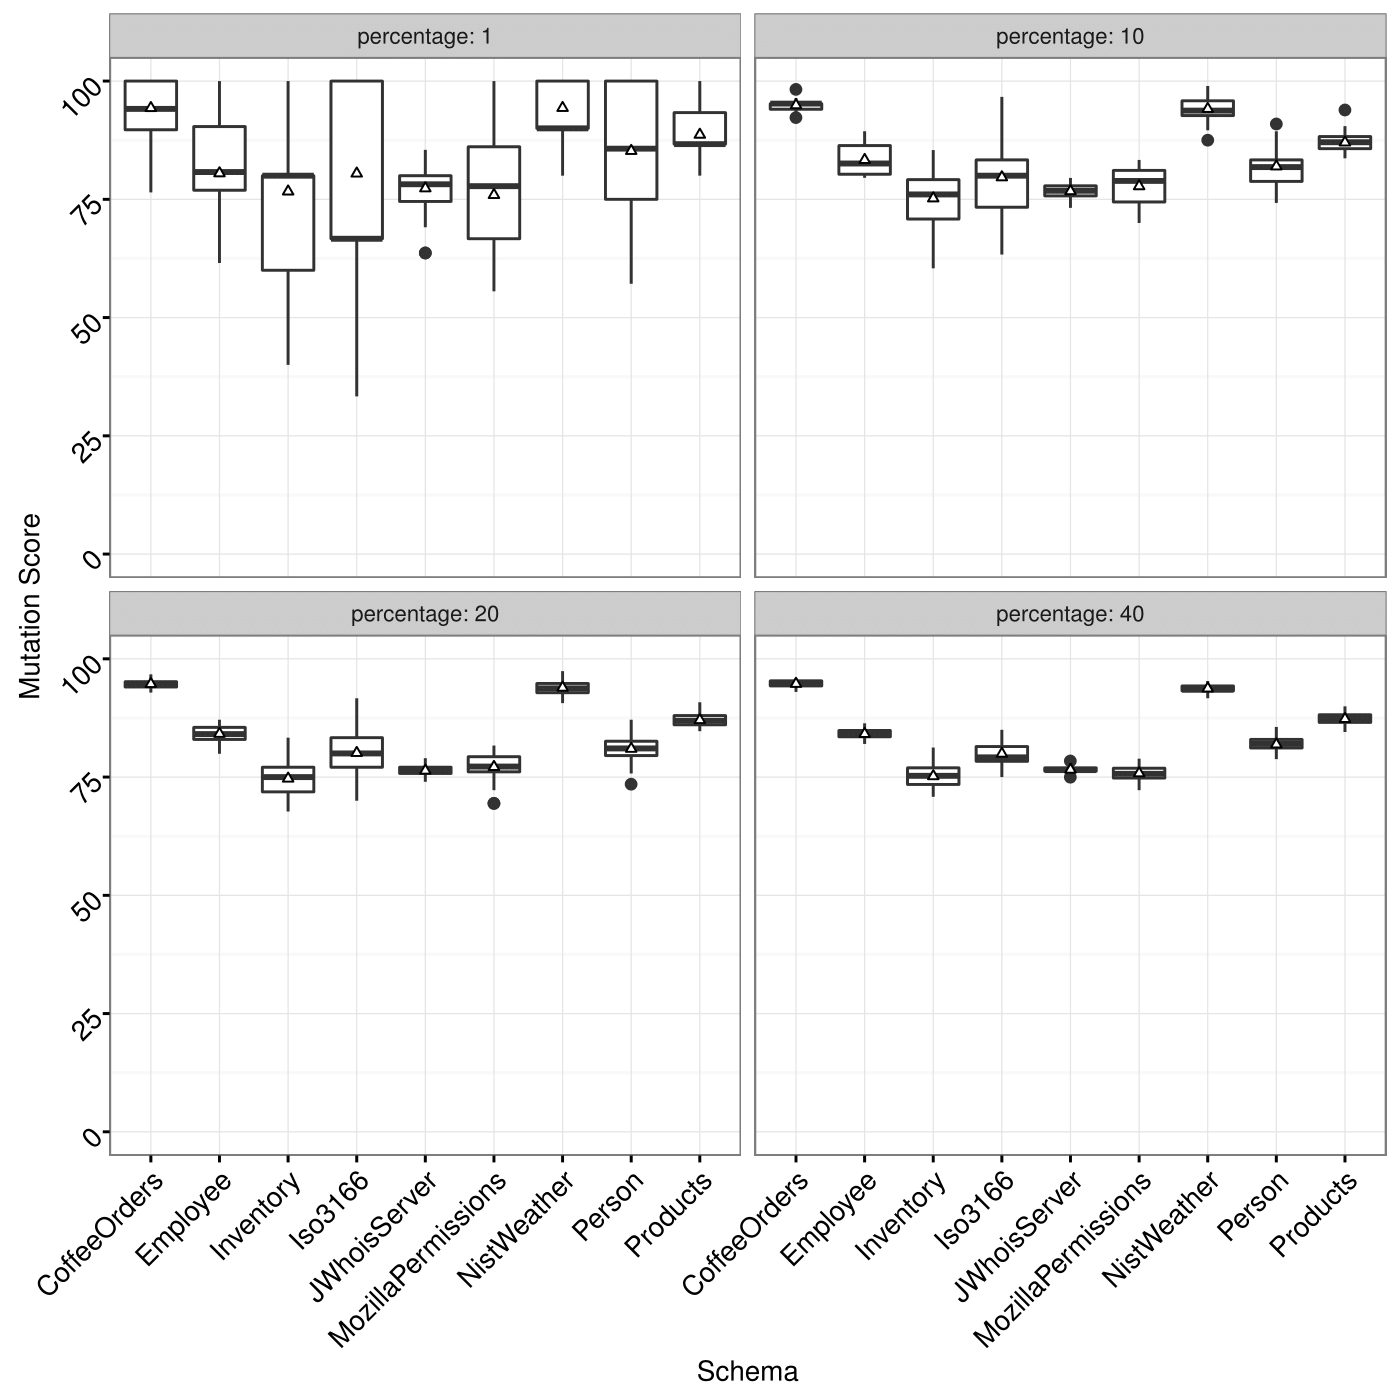
\includegraphics[scale=0.14]{mutation_score_random_plot.png}
  \end{frame}


\section{Results}
  \begin{frame}
    \frametitle{Results}
    \centering
    \fontsize{90}{72}\selectfont
    10\%
  \end{frame}


\section{Conclusion}
  \begin{frame}
    \frametitle{Conclusion}
    % I don't like how the bullets are not in the middle of the word
    \centering
    \begin{HUGE}
    \begin{itemize}
        \item \visible<1->{Mutation Testing}
        \item \visible<2->{Limitations}
        \item \visible<3->{mrstudyr}
        \item \visible<4->{Comparable}
    \end{itemize}
    \end{HUGE}
  \end{frame}


% \section{Future Work}
%   \begin{frame}
    \frametitle{Future Work}
    \centering
    \begin{tikzpicture}[node distance=0cm, auto,>=stealth, thick]


    \tikzstyle{box}=[rectangle, draw=solarizedBase02, rounded corners, fill=solarizedBlue, drop shadow,
            text centered, anchor=north, text=white, minimum height = 0.6cm, text width=10cm]
    \tikzstyle{boxv}=[rectangle, draw=solarizedBase02, rounded corners, fill=solarizedOrange, drop shadow,
            text centered, anchor=north, text=white, minimum height = 0.6cm, text width=8cm]

            \visible<1->{\node (programs) [box] {Extend to Programs};}
            \visible<2->{\node (approaches) [box, below = 0.6cm of programs] {Additional Reduction Techniques};}
            % \visible<3->{\node (mutation) [box, below = 0.6cm of testsuite] {Mutation Testing};}
            % \visible<4->{\node (reduction) [box, below = 0.6cm of mutation] {Reduction Techniques};}
            % \visible<5->{\node (retrospective) [boxv, below = 0.6cm of reduction] {mrstudyr};}

            % \visible<2->{\draw[->, line width = 4pt] (quality) -- (testsuite);}
            % \visible<3->{\draw[->, line width = 4pt] (testsuite) -- (mutation);}
            % \visible<4->{\draw[->, line width = 4pt] (mutation) -- (reduction);}
            % \visible<5->{\draw[->, line width = 4pt] (reduction) -- (retrospective);}

\end{tikzpicture}

  \end{frame}


\section{Grand Finale}
  \begin{frame}
      % TODO: fix the weird spacing on this slide
    \frametitle{Grand Finale}
    \begin{columns}
    \begin{column}{0.5\textwidth}
        \centering
        \visible<1->{\begin{tikzpicture}[node distance=0cm, auto,>=stealth, thick]

    \tikzstyle{mutant}=[rectangle, draw=solarizedBase02, rounded corners, fill=white, drop shadow,
            text centered, anchor=north, text=white, minimum height = 0.2cm, text width=0.1cm]
    \tikzstyle{mutantviolet}=[rectangle, draw=solarizedBase02, rounded corners, fill=solarizedViolet, drop shadow,
            text centered, anchor=north, text=white, minimum height = 0.2cm, text width=0.1cm]
    \tikzstyle{mutantred}=[rectangle, draw=solarizedBase02, rounded corners, fill=solarizedRed, drop shadow,
            text centered, anchor=north, text=white, minimum height = 0.2cm, text width=0.1cm]
    \tikzstyle{mutantblue}=[rectangle, draw=solarizedBase02, rounded corners, fill=solarizedBlue, drop shadow,
            text centered, anchor=north, text=white, minimum height = 0.2cm, text width=0.1cm]
    \tikzstyle{mutantorange}=[rectangle, draw=solarizedBase02, rounded corners, fill=solarizedOrange, drop shadow,
            text centered, anchor=north, text=white, minimum height = 0.2cm, text width=0.1cm]
    \tikzstyle{mutantlightblue}=[rectangle, draw=solarizedBase02, rounded corners, fill=solarizedBlue!25, drop shadow,
            text centered, anchor=north, text=white, minimum height = 0.2cm, text width=0.1cm]
    \tikzstyle{mutantlightorange}=[rectangle, draw=solarizedBase02, rounded corners, fill=solarizedOrange!25, drop shadow,
            text centered, anchor=north, text=white, minimum height = 0.2cm, text width=0.1cm]
    \tikzstyle{operator}=[rectangle, draw=solarizedBase02, rounded corners, fill=solarizedOrange, drop shadow,
            text centered, anchor=north, text=white, minimum height = 1cm, text width=8cm]
    \tikzstyle{box}=[rectangle, draw=solarizedBase02, rounded corners, fill=solarizedBlue, drop shadow,
            text centered, anchor=north, text=white, minimum width = 3cm, minimum height = 1.5cm, text width=3cm]

  \visible<1->{
    \foreach \x in {1,3,5}
    \foreach \y in {1,3,5}
       {\pgfmathtruncatemacro{\label}{\x - 3 *  \y + 30}
   \node [mutantblue]  (\x\y) at (0.5*\x,0.5*\y) {};}}

  \visible<1->{
    \foreach \x in {0,2,4,6}
    \foreach \y in {0,2,4,6}
       {\pgfmathtruncatemacro{\label}{\x - 3 *  \y + 30}
   \node [mutantred]  (\x\y) at (0.5*\x,0.5*\y) {};}}

  \visible<2->{
  \node [box] at (1.5,-1) {\LARGE Reduced};}

\end{tikzpicture}
}
    \end{column}
    \hfill%
    \begin{column}{0.6\textwidth}
        \centering
        \visible<2->{\fontsize{90}{72}\selectfont 10\%}
        \visible<3->{\textcolor{solarizedBase02}{\rule{0.8\textwidth}{2pt}}}
        \visible<3->{\textcolor{solarizedOrange}{\href{https://github.com/mccurdyc/mrstudyr}{\fontsize{90}{72}{\faGithub}}}}
    \end{column}
    \end{columns}
    \end{frame}


\end{document}
